% !TeX encoding = windows-1251
\documentclass[fullscreen=true,russian,compress,%
	hyperref={unicode,bookmarks=false}]{presentation}
\inputencoding{utf8} % Кодировка вашего файла
% Внимание! Опция russian не совместима с \tableofcontents
\usepackage[russian]{babel} % Эту строку можно удалить
\usepackage{paratype} % Выбираем шрифт
% Определяем длины частей нижнего колонтитула: автор, название, число слайдов
\makefootline{.35}{.55}{.1} % Сумма длин = 1

\usepackage{tikz} % Для создания рисунков с помощью tikz
\usepackage{listings} % Для листингов программ

\begin{document}

% Если потребуется, переводим названия блоков с английского:
\deftranslation[to=Russian]{Theorem}{Теорема}
\deftranslation[to=Russian]{Example}{Пример}

% Данные титульного слайда
\title[Методы обратной свертки в задачах космической физики]{Методы обратной свертки в задачах \\ космической физики}
\author{Ющенко Александр Владиславович}
\institute{Научный руководитель: Ю.\,В.~Богомолов}
\date{27.06.2023}

% Создаем титульный слайд
\begin{frame}
\titlepage
\end{frame}

% \tableofcontents не работает при включенной опции russian пакета babel
%\begin{frame}{Содержание}\tableofcontents\end{frame}

\section{Вступление}


\begin{frame}{Задача обратной свертки}
   \begin{figure}[!ht]
      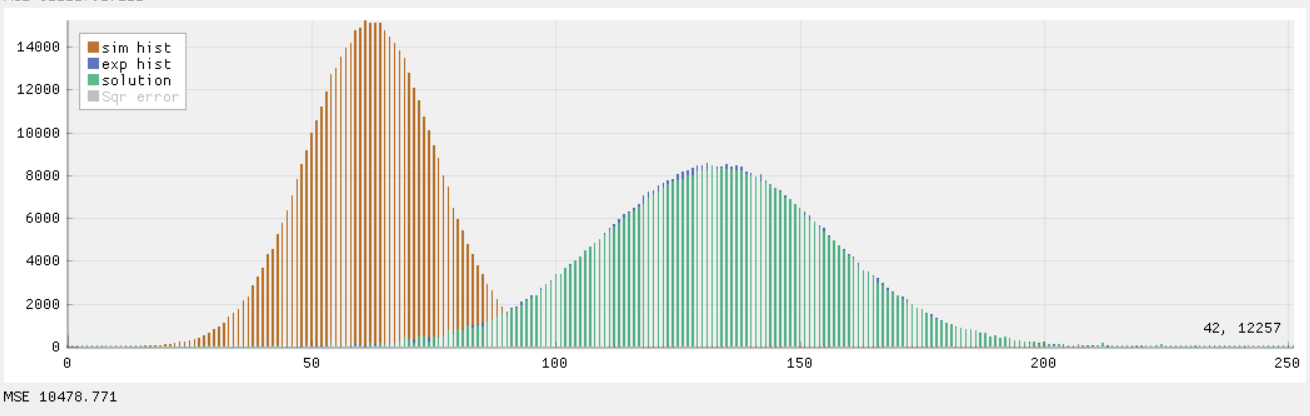
\includegraphics[width=\linewidth]{images/example_regulazation.png}
   \end{figure}
\end{frame}

\begin{frame}{Задача обратной свертки}
\begin{block}{}
   Разделим множество значений исходной величины на интервалы 
   $(\Delta_{1}, \Delta_{2}, \cdots ,\Delta_{n_{\tau}})$. Дискретным распределением величины будем называть вероятности попадания 
   в определенный интервал $p = (p_{1}, p_{2}, \cdots, p_{n_{\tau}})$. Измеренный спектр обозначим $m = (m_{1}, m_{2}, \cdots, m_{n_{m}})$.
   Предполагаемый истинный спектр - $\tau$ размерности $n_{\tau}$.
\end{block}
\begin{block}{}
   Описание искажений определяется матрицей миграций, которая определят вероятность попадания случайный величины в какой-то бин при 
   условии что истинное значение попадает в свой бин.
   Это дает нам систему линейных отношений между смоделированным истинным и измеренным распределениями: 
   \begin{equation}
      A\tau = m
   \end{equation}
\end{block}
\end{frame}

\begin{frame}{Матрица миграций}
   Матрица $A$ размера $n_{m} \times n_{\tau}$ строится следующим образом:
   $A_{ij} = P( \text{ измеренное } \in \text{Bin}_{i} \mid \text{ истинное } \in \text{Bin}_{j} )$
\begin{figure}[!ht]
   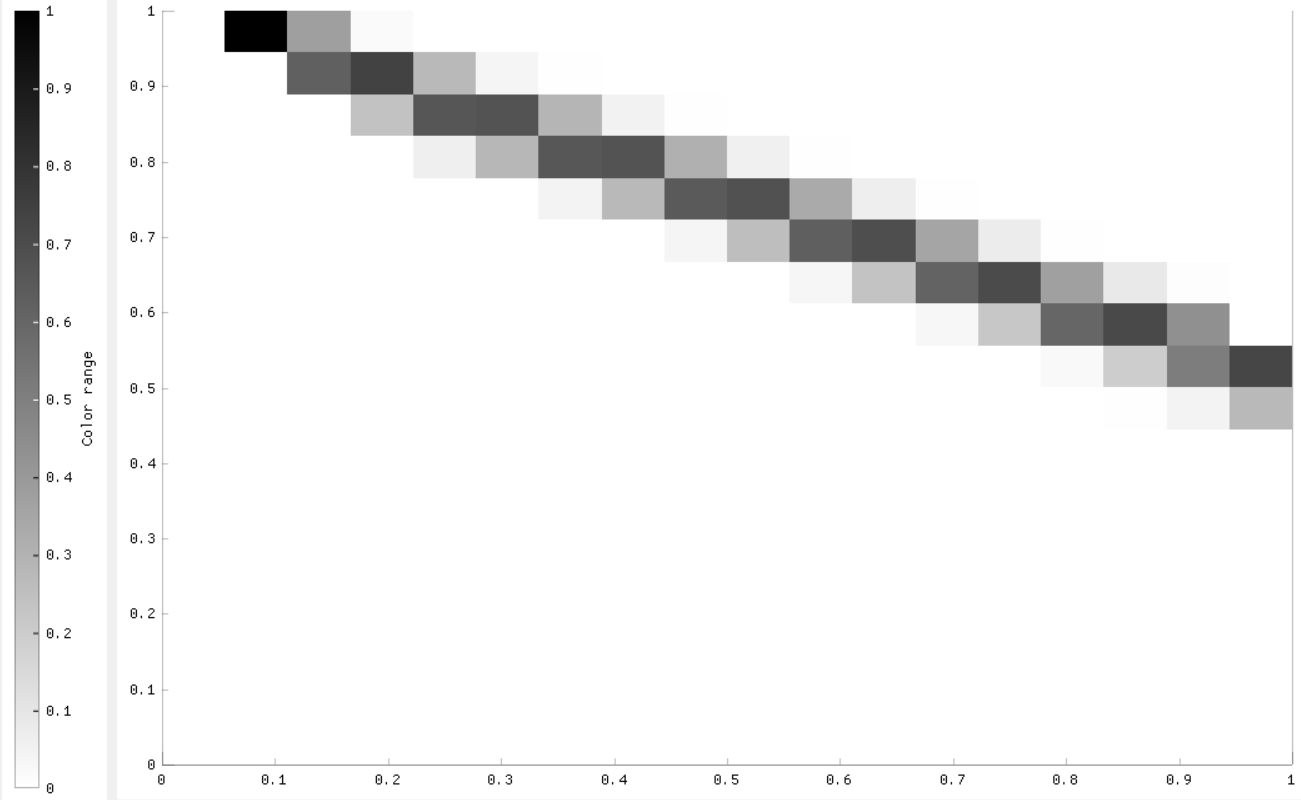
\includegraphics[scale=0.3]{images/gaus_mig_black.png}
\end{figure}
\end{frame}



\begin{frame}{Метод регуляризации}
\begin{block}{}
   Задача минимизации для прямого подхода:
   \begin{equation}
      \Phi(\tau)=(R\tau-m)^T (R\tau-m) \to min_{\tau}
      \label{min_base}
   \end{equation}
\end{block}
\begin{block}{}
   Для того, чтобы учитывать дополнительно характер распределения, предлагается добавить регуляризационное слагаемое  
   которое может описывать, например, гладкость. С учетом дополнительного слагаемого система будет иметь следующий вид: 

   \begin{equation}
      \Phi(\tau)=(R\tau-m)^T (R\tau-m) + \alpha S(\tau) \to min_{\tau}
      \label{min_svd}
   \end{equation}

   Здесь S(τ ) как раз играет роль регуляризатора, а α - это коэффициент сгла-
   живания. Соответственно при \alpha = 0 получаем исходную систему
\end{block}
\end{frame}


% \begin{frame}{Решение задачи обратной свертки методом регуляризации в одномерном случаи}

% Для одномерного случая соседство определяется естественным образом, бины записываются последовательно, и соседними считаются, те бины, номер 
% которых отличается на единицу. В качестве регуляризационного слагаемого из задачи минимизации \eqref{min_svd} предлагаться брать следующую функцию:
% \begin{equation}
%     S(\tau)= \sum_{i=2}^{n-1} (\tau_{i-1} - 2\tau_{i} + \tau_{i+1})^2
% \end{equation}

% Которая отражает гладкость искомого распределения и является суммой квадратов второй производной по всем интервалам дискретизации. 
% Она также может быть записана в матричном виде:
% \end{frame}

\begin{frame}{Решение задачи обратной свертки методом регуляризации в одномерном случаи}

   \begin{equation}
      S(\tau) = (C\tau)^T(C\tau)
  \end{equation}
 
  где матрица $C$ определяет соседство бинов и имеет следующий вид:

   \begin{equation}
       C_{m,n} = 
    \begin{pmatrix}
      \quad 1 &       -1 &  \quad 0 &  \quad 0 & 0 & \cdots & 0 \\
           -1 &  \quad 2 &       -1 &  \quad 0 & 0 & \cdots & 0 \\
            0 &       -1 & \quad  2 &       -1 & 0 & \cdots & 0 \\
     \vdots &  & & \ddots & & & \vdots \\
     0  & 0  & 0 & 0 & \cdots & -1 & 1
    \end{pmatrix}
    \label{one_dim_neighbors_mat}
   \end{equation}

   Теперь мы можем переписать задачу минимизации \eqref{min_svd} следующих образом:
   \begin{equation}
      \Phi(\tau)=(R\tau-m)^T (R\tau-m) + \alpha(C\tau)^T(C\tau) \to min_{\tau}
      \label{min_one_dim}
   \end{equation}
\end{frame}


\begin{frame}{Решение задачи обратной свертки методом регуляризации в одномерном случаи}
Данную задачу минимизации можно переопределить в виде расширенной системы линейных уравнений:
\begin{equation}
       \begin{bmatrix}
           RC^{-1} \\
           \sqrt{a} \cdot I
       \end{bmatrix}
       C\tau = 
       \begin{bmatrix}
           m \\
           0
       \end{bmatrix}
       \label{system_one_dim}
   \end{equation}
После, следуя алгоритму, можно получить точное решения слау:
\begin{enumerate}
    \item Выполняем сингулярное разложение матрицы A \\
    $USV^T \tau = m.$
    \item Делаем замену $z = V^T\tau$. Получаем $USz = m.$
    \item $U$ - ортогональная, это значит что обратная матрица ровна транспонированной. Домножая систему на $U^{-1}$ получаем $Sz=U^Tm$.
    \item Далее делаем замену $d=U^Tm$, и система принимает вид $Sz=d$.
    \item Отсюда находим $z_{i} = \frac{d_{i}}{s_{i}} \cdot \frac{s^2_{i}}{s^2_{i} + \alpha}$.
    \item Решение системы находим находим следующим образом $\tau = Vz$.
\end{enumerate}
\end{frame}


\begin{frame}{Решение задачи обратной свертки методом регуляризации в многомерном случаи}
   Матрица $C$ является подмножеством матрицы $K$, и для нового слагаемого можно вводить более сложные
   отношения соседства. Во первых, близкими могут быть бины у которых не только общая грань, а во вторых, сила связи для разных бинов
   может отличаться. Для силы связи введем параметр $\omega(\Delta_{i}, \Delta_{j}) \geq 0$ - который описывает вес соседних ячеек. 
   Теперь постоим матрицу, с не бинарным отношением:
   \begin{equation}
    k_{ij} =
     \begin{cases}
       \displaystyle\sum_{k\neq i} w(\Delta_{i}, \Delta_{k}), \text{ при } \ i = j \\
       -w( \Delta_{i}, \Delta_{j} ), \text{ при } i \neq j
     \end{cases}
   \end{equation}
   \begin{equation}
      \Phi(\tau)=(R\tau-m)^T (R\tau-m) + \alpha(K\tau)^T(K\tau) \to min_{\tau}
      \label{min_n_dim}
   \end{equation}
\end{frame}


\begin{frame}{Небинарное отношение соседства}
   \begin{enumerate}
      \item Можно учитывать площадь соприкосновения двух соседних бинов или их размеры
      \item Учитывать при вычислении силы связи через расстояния центров масс бинов
      \item Вычислять основываясь на количество элементов истинного спектра попавших в данный бин
      \begin{enumerate}
         \item  $k_{ij} = - count_(\Delta_{i}, \Delta_{j}) \cdot neighobrs(\Delta_{i}, \Delta_{j})$ \\
         \item  $k_{ii} = \displaystyle\sum_{j} k_{ij}$ \\
         \item  $k_{ij} = \frac{k_{ij}}{k_{ii}}$
      \end{enumerate}
      Где $count(\Delta_{i}, \Delta_{i})$ - функция, описывающая, количество измеренных значений попавших в $j$ бин. 
      И $neighbors(\Delta_{i}, \Delta_{j})$ - функция возвращающая 1 если два бина являются соседями и 0 в противном случаи.
   \end{enumerate}
\end{frame}


\begin{frame}{Бининг}
   \begin{figure}[h!]
      \centering
      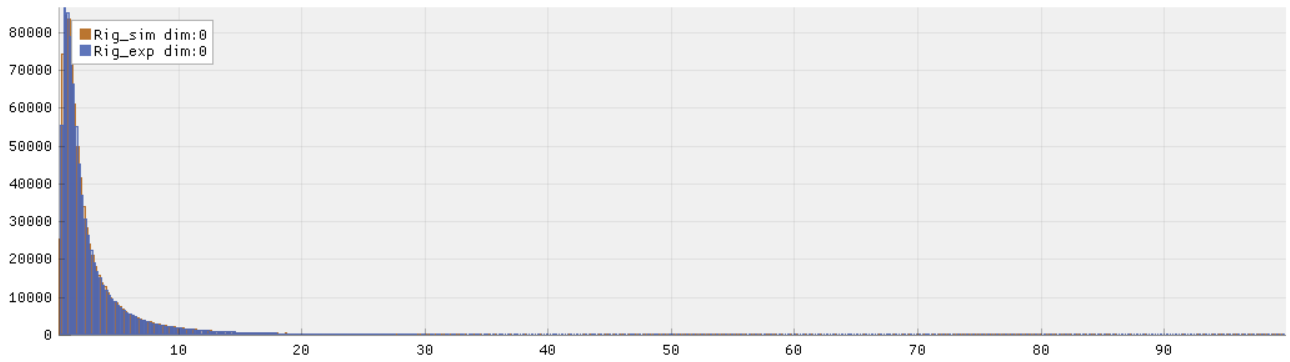
\includegraphics[width=\linewidth]{images/rig_dist.png}
      \caption{Гистограма для истинных и измеренных значений жесткости}
      \label{photo:rig_dist}
   \end{figure}
   \begin{figure}[h!]
      \centering
      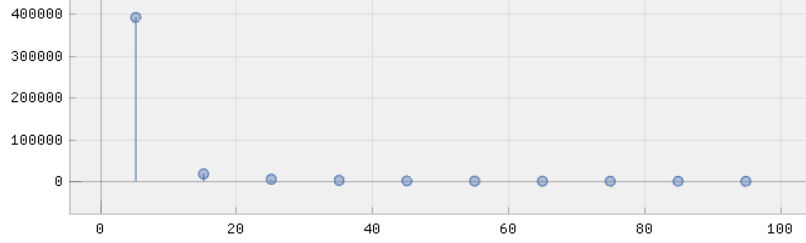
\includegraphics[scale=0.55]{images/rig_static_binning.png}
   \end{figure}
\end{frame}


% \begin{frame}{Бининг}
%    \begin{enumerate}
%       \item Разбиение области значений на равные интервалы \\ (Статический биннинг)
%       \item Последовательно делим интервалы, с наибольшим числом элементов, на два разных, проводя границу 
%       по центру исходного \\ (Динамический биннинг )
%       \item Последовательно делим интервалы, с наибольшим числом элементов, на два разных, проводя границу 
%       по медиане, то есть середине отсортированного вектора элементов \\ (Динамический медианный биннинг)
%       \item Часть интервалов строим строим статически, далее используем динамический подход \\ (Гибридный биннинг)
%    \end{enumerate}
% \end{frame}

\begin{frame}{Биннинг}
   \begin{figure}[h!] 
      \centering
      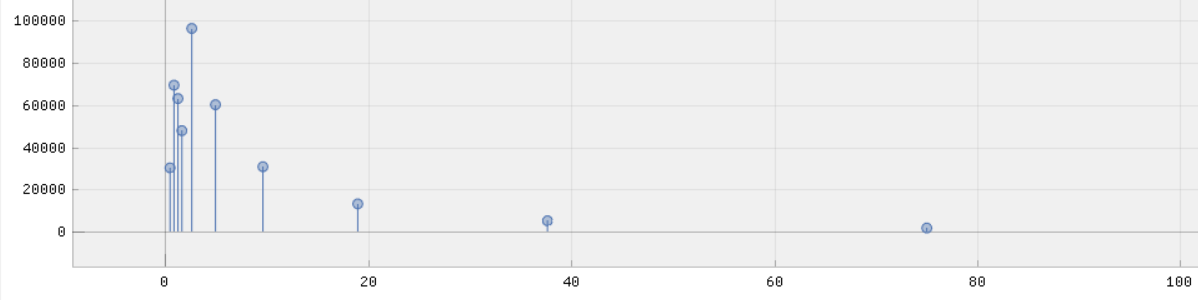
\includegraphics[scale=0.37]{images/rig_dynamic_binning.png}
   \end{figure}
   \begin{figure}[h!]
      \centering
      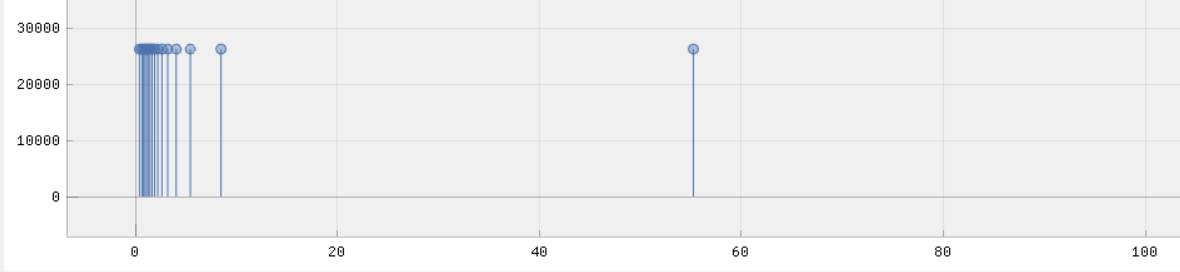
\includegraphics[scale=0.37]{images/rig_median_binning.png}
   \end{figure}
   \begin{figure}[h!]
      \centering
      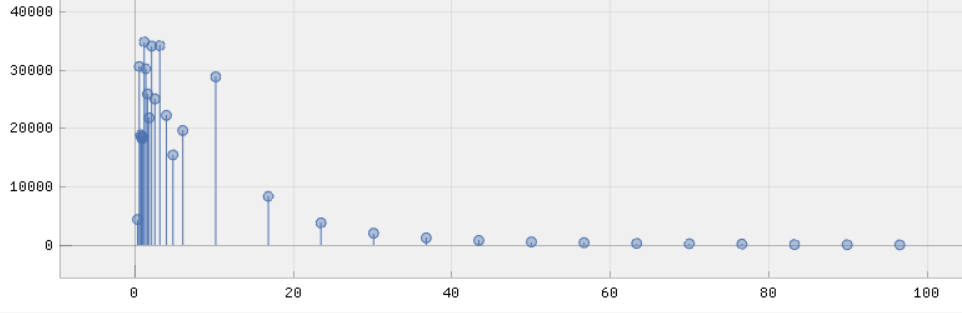
\includegraphics[scale=0.46]{images/hybrid_binningpng.png}
   \end{figure}
\end{frame}


\begin{frame}{Результаты}
   \begin{figure}[h!]
      \centering
      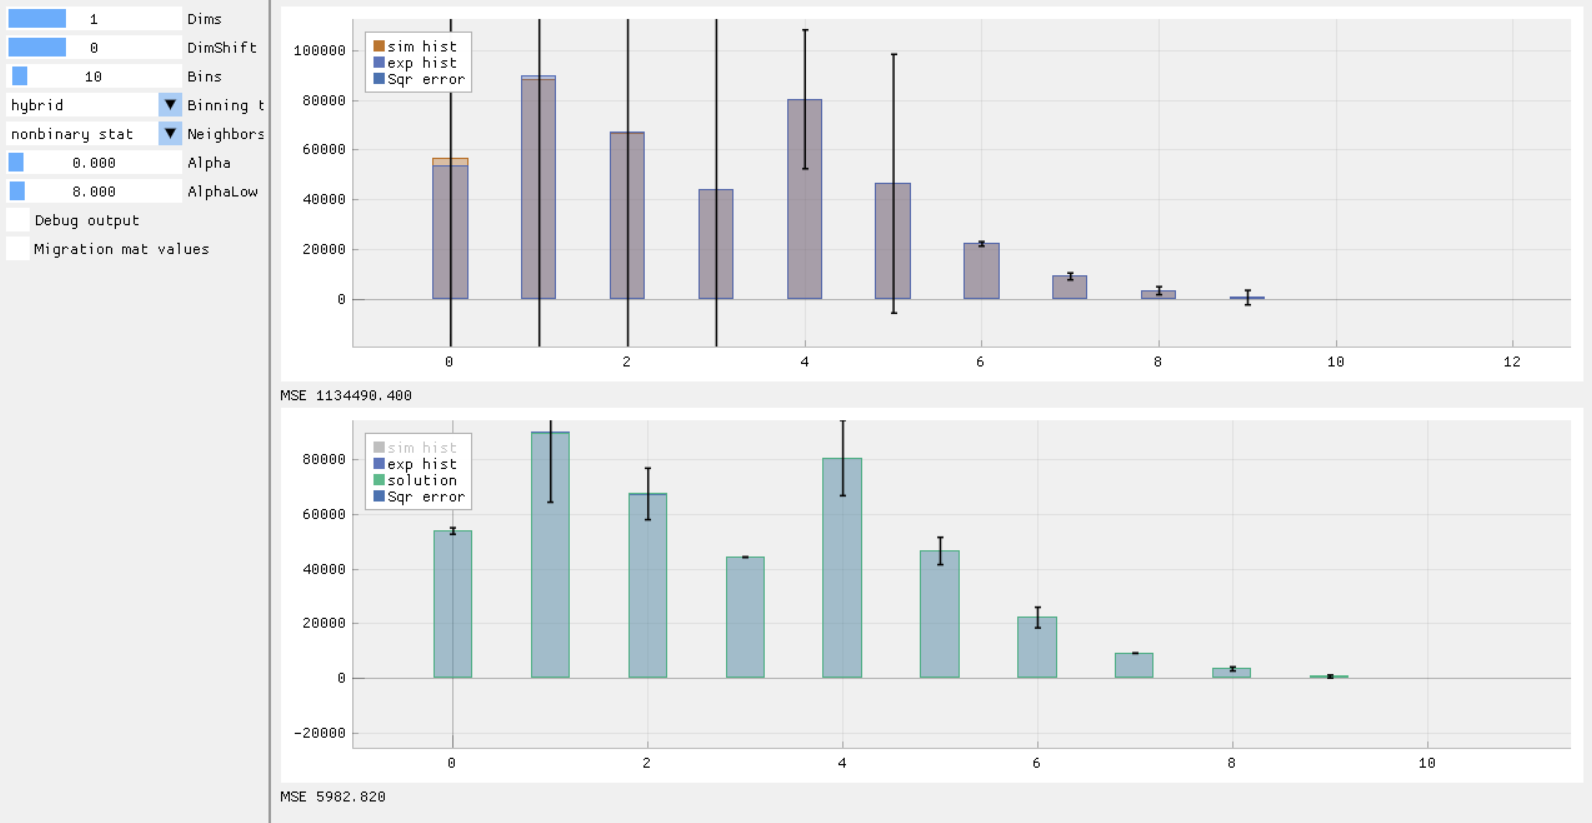
\includegraphics[width=\linewidth]{images/1d_rig_res.png}
      \caption{Одномерный случай. Жесткость частицы}
   \end{figure}
   
\end{frame}


\begin{frame}{Результаты}
   \begin{figure}[h!]
      \centering
      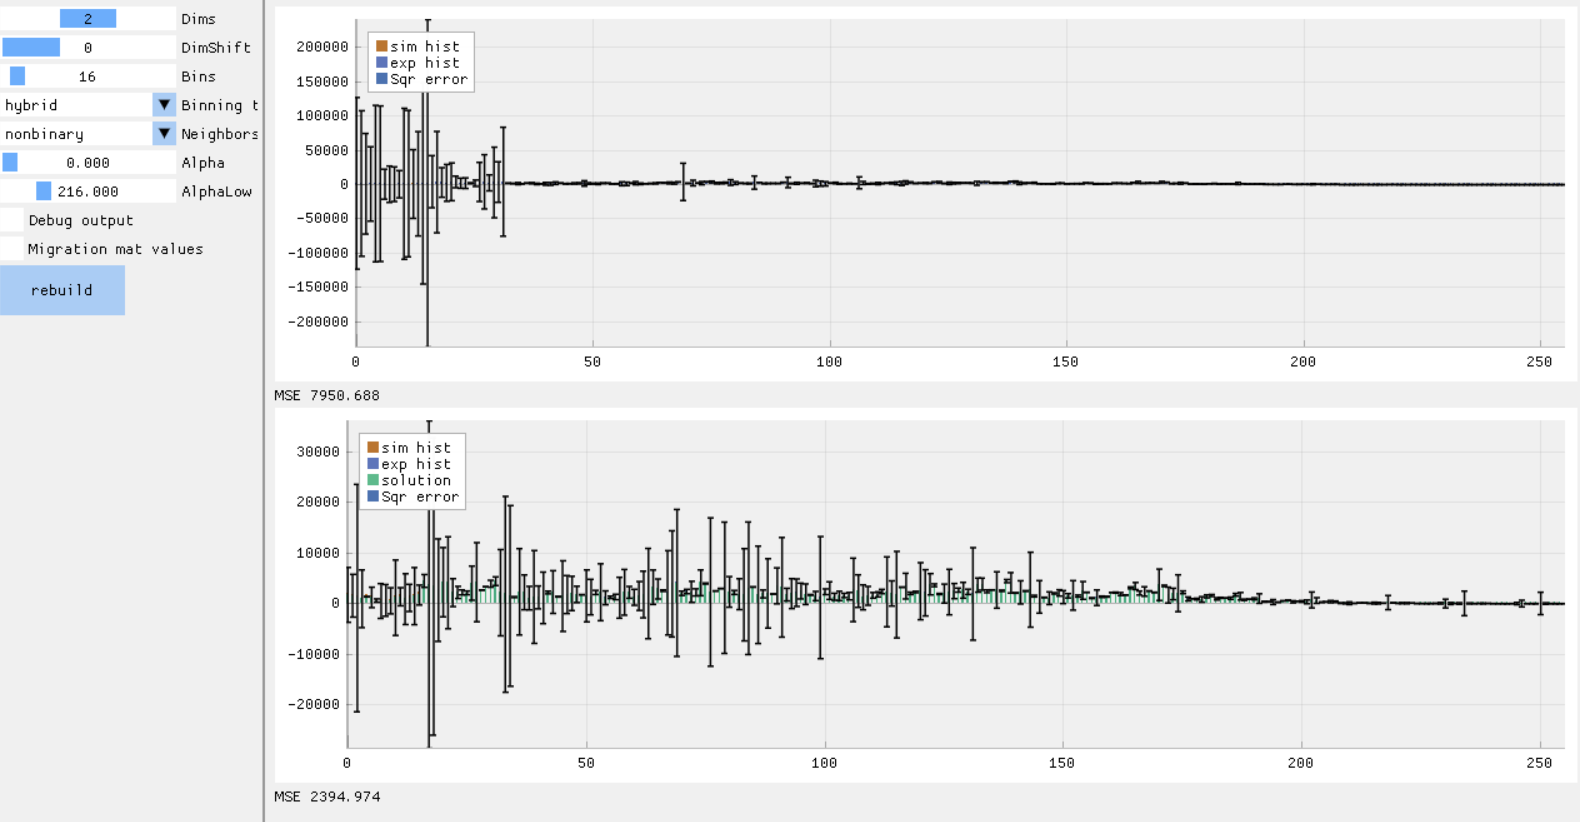
\includegraphics[width=\linewidth]{images/2d_rig_azim_res.png}
      \caption{Двумерный случай. Жесткость и полярный угол}
   \end{figure}
\end{frame}

\begin{frame}{Итог}
   \begin{enumerate}
      \item Было разработано приложение позволяющее автономно решать задачу обратной свертки в многомерном случаи.
      \item Проверена идея решения многомерной задачи через n одномерных.
      \item Рассмотрены решения задачи автоматизированной дискретизации.
      \item Рассмотрены не бинарные отношения соседства для регуляризационного слагаемого.
   \end{enumerate}
\end{frame}

\end{document}

